\documentclass[12pt,a4paper,twoside]{report}
% -------------------------------------------------------------------- %
% Pacotes

\usepackage[utf8]{inputenc}
\usepackage[T1]{fontenc}
\usepackage[brazil]{babel}
\usepackage[fixlanguage]{babelbib}
\usepackage[pdftex]{graphicx}      % usamos arquivos pdf/png como figuras
\usepackage{setspace}              % espaçamento flexvel
\usepackage{indentfirst}           % indentação do primeiro parágrafo
\usepackage{makeidx}               % índice remissivo
\usepackage[nottoc]{tocbibind}     % acrescentamos a bibliografia/indice/conteudo no Table of Contents
\usepackage{courier}               % usa o Adobe Courier no lugar de Computer Modern Typewriter
\usepackage{type1cm}               % fontes realmente escaláveis
\usepackage{titletoc}
\usepackage{ucs}
\usepackage[font=small,format=plain,labelfont=bf,up,textfont=it,up]{caption}
\usepackage[usenames,svgnames,dvipsnames]{xcolor}
\usepackage[a4paper,top=2.54cm,bottom=2.0cm,left=2.0cm,right=2.54cm]{geometry} % margens
\usepackage{amsmath}
\usepackage{booktabs} % cria tabelas em formato profissional
\usepackage[pdftex,plainpages=false,pdfpagelabels,pagebackref,colorlinks=true,citecolor=DarkGreen,
linkcolor=NavyBlue,urlcolor=DarkRed,filecolor=green,bookmarksopen=true]{hyperref} % links coloridos
\usepackage[all]{hypcap}                % soluciona o problema com o hyperref e capítulos
\usepackage[square,sort,nonamebreak,comma]{natbib}  % citação bibliográfica alpha
\fontsize{60}{62}\usefont{OT1}{cmr}{m}{n}{\selectfont}
\usepackage{upquote}                    % formata apóstrofes '
\usepackage{textcomp}

% Para formatar corretamente as URLs
\usepackage{url}
% -------------------------------------------------------------------- %
% Cabeçalhos similares ao TAOCP de Donald E. Knuth
\usepackage{fancyhdr}
\pagestyle{fancy}
\fancyhf{}
\renewcommand{\chaptermark}[1]{\markboth{\MakeUppercase{#1}}{}}
\renewcommand{\sectionmark}[1]{\markright{\MakeUppercase{#1}}{}}
\renewcommand{\headrulewidth}{0pt}

\frenchspacing                     % arruma o espaço: id est (i.e.) e exempli gratia (e.g.)
\urlstyle{same}                    % URL com o mesmo estilo do texto e no mono-spaced
\makeindex                         % para o índice remissivo
\raggedbottom                      % para no permitir espaços extras no texto
\fontsize{60}{62}\usefont{OT1}{cmr}{m}{n}{\selectfont}
\cleardoublepage
\normalsize

% -------------------------------------------------------------------- %
% Cores para formatação de código
\usepackage{color}
\definecolor{vermelho}{rgb}{0.6,0,0} % para strings
\definecolor{verde}{rgb}{0.25,0.5,0.35} % para comentários
\definecolor{roxo}{rgb}{0.5,0,0.35} % para palavras-chaves
\definecolor{azul}{rgb}{0.25,0.35,0.75} % para strings
\definecolor{cinza-claro}{gray}{0.95}
% -------------------------------------------------------------------- %
% Opções de listagem usados para o código fonte
% Ref: http://en.wikibooks.org/wiki/LaTeX/Packages/Listings
\usepackage{listings}           % para formatar código-fonte (ex. em Java)

\lstset{ %
language=Python,                      % seleciona a linguagem do código
basicstyle=\footnotesize\ttfamily,    % o tamanho da fonte usado no código
commentstyle=\color{verde}\bfseries,  % formatação de comentários
stringstyle=\color{azul},             % formatação de strings
upquote=true,
numbers=left,                   % onde colocar os números de linha
numberstyle=\tiny,  % o tamanho da fonte usada para a numeração das linhas
stepnumber=1,                   % o intervalo entre dois números de linhas. Se for 1, numera cada uma.
numbersep=5pt,                  % how far the line-numbers are from the code
showspaces=false,               % show spaces adding particular underscores
showstringspaces=false,         % underline spaces within strings
showtabs=false,                 % show tabs within strings adding particular underscores
keywordstyle=\color{roxo}\bfseries,
keywordstyle=[1]\color{roxo}\bfseries,
keywordstyle=[2]\color{verde}\bfseries,
frame=b,                   % adds a frame around the code
framerule=0.6pt,
tabsize=2,                      % sets default tabsize to 2 spaces
captionpos=t,                   % sets the caption-position to top
breaklines=true,                % sets automatic line breaking
breakatwhitespace=false,        % sets if automatic breaks should only happen at whitespace
escapeinside={\%*}{*)},         % if you want to add a comment within your code
backgroundcolor=\color[rgb]{1.0,1.0,1.0}, % choose the background color.
rulecolor=\color[rgb]{0.8,0.8,0.8},
extendedchars=true,
xleftmargin=10pt,
xrightmargin=10pt,
framexleftmargin=10pt,
framexrightmargin=10pt,
literate={â}{{\^{a}}}1  % para formatar corretamente os acentos do Português ao usar utf8
    {ê}{{\^{e}}}1
    {ô}{{\^{o}}}1
    {Â}{{\^{A}}}1
    {Ê}{{\^{E}}}1
    {Ô}{{\^{O}}}1
    {á}{{\'{a}}}1
    {é}{{\'{e}}}1
    {í}{{\'{i}}}1
    {ó}{{\'{o}}}1
    {ú}{{\'{u}}}1
    {Á}{{\'{A}}}1
    {É}{{\'{E}}}1
    {Í}{{\'{I}}}1
    {Ó}{{\'{O}}}1
    {Ú}{{\'{U}}}1
    {à}{{\`{a}}}1
    {À}{{\`{A}}}1
    {ã}{{\~{a}}}1
    {õ}{{\~{o}}}1
    {Ã}{{\~{A}}}1
    {Õ}{{\~{O}}}1
    {ç}{{\c{c}}}1
    {Ç}{{\c{C}}}1
    {ü}{{\"u}}1
    {Ü}{{\"U}}1
}

\renewcommand{\lstlistingname}{Listagem}
\renewcommand{\lstlistlistingname}{Lista de Listagens}

% \captionsetup[lstlisting]{singlelinecheck=false, labelfont={blue}, textfont={blue}}
\usepackage{caption}
\DeclareCaptionFont{white}{\color{white}}
\DeclareCaptionFormat{listing}{\colorbox[cmyk]{0.43, 0.35, 0.35,0.01}{\parbox{\textwidth}{\hspace{15pt}#1#2#3}}}
\captionsetup[lstlisting]{format=listing,labelfont=white,textfont=white, singlelinecheck=false, margin=0pt, font={bf,footnotesize}}

\title{Análise experimental de algoritmos usando Python}
\author{Patrícia Mariana Ramos Marcolino \\
\texttt{\small \url{pmrmarcolino@hotmail.com}}
\vspace{1cm} \\
Eduardo Pinheiro Barbosa\\
\texttt{\small \url{eduardptu@hotmail.com}}
\vspace{1cm} \\
Faculdade de Computação \\
Universidade Federal de Uberlândia
}
\date{\today}

\begin{document}
\maketitle
% -------------------------------------------------------------------- %
% Listas de figuras, tabelas e códigos criadas automaticamente
\listoffigures
\listoftables
\lstlistoflistings
% -------------------------------------------------------------------- %

% -------------------------------------------------------------------- %
% Sumário
\tableofcontents
% cabeçalho para as páginas de todos os capítulos
\fancyhead[RE,LO]{\thesection}

%\singlespacing              % espaçamento simples
\setlength{\parskip}{0.15in} % espaçamento entre paragráfos

\chapter{Análise}
\subsection{Desempenho do quicksort no pior caso}
Podemos supor que o {\it partition} não consome mais que $5n+6$ unidades de tempo, sendo $n=r-p+1$. Então o consumo de tempo do {\it quicksort} no pior caso, digamos $T(n)$, satisfaz a seguinte recorrência \[T(n) = 5n+7+ max _{\text{0} \leq \text{k} \leq \text{n}} (T(k)+T(n-k)\]
onde o máximo é tomado sobre todos os possíveis valores de k no intervalos 1.. $n-1$. Podemos supor $T(1)=1$. Assim, por exemplo, $T(2)\leq 10+7+T(1)+T(1)= 19$. Em geral, vamos mostrar que \[T(n) \leq 5n^2\]
para $n = 1,2,3,...$ a desigualdade é certamente verdadeira quando $n=1,2,3$. Agora suponha que $n>3$ e suponha que a desigualdade vale para $T(i)$ sempre que $i<n$. Teremos então

\[T(n) = 5n+7+max_{k} (T(k) + T(n-k))\]
\[\leq 5n+7+max_{k} (5*k^2+5(n-k)^2)\]
\[= 5n+7+5(1 + T(n-1)^2)\]
\[= 5*n^2 - 5*n+17\]
\[\leq 5*n^2\]

O terceiro passo da prova segue da seguinte observação: para $n$ fixo e $k$ variando entre 1 e $n-1$, a expressão $k^2+(n-k)^2$ tem valor máximo nos pontos $k = 1$ e $k=n-1$ (e atinge o mínimo quando $k$ está próximo de $n/2$). O último passo da prova está correto pois quando $n>3$ tem-se $-5*n+17 \leq0$.

A recorrência pode ser reescrita como $T(n) = 5n+7+ max _{\text{0} \leq \text{k} \leq \text{n}} (T(k)+T(n-k) + O(n)$ daí se deduz que $T(n)$ está em $O(n^2)$. Conclusão: no pior caso, o algoritmo {\it quickSort} é quadratico.  

\subsection{Desempenho típico e melhor caso do quicksort}

O melhor desempenho do Quicksort ocorre quando todas as invocações de {\it partition} dividem o vetor na proporção $(1/2)$-para-$(1/2)$, ou seja, quando todas as invocações devolvem um índice que está a meio caminho entre $p$ e $r$.  O consumo de tempo do algoritmo nesse caso, digamos $S(n)$, satisfaz a recorrência
\[S(n) = S(\lceil{}n/2\rceil{})+S(\lfloor{}n/2\rfloor{}) + 5*n + 7\] 

para todo natural $n \geq 2$, podemos mostrar que
\[S(n) \leq 12*n\log_{2}n\]
para todo natural $n \geq 3$

O comportamento não é muito diferente quando o vetor é dividido de maneira menos equilibrada.  Suponha, por exemplo, que todas as invocações de Separe dividem o vetor na proporção $(1/9)$-para-$(8/9)$.  Nesse caso, o consumo de tempo, digamos $R(n)$, satisfaz recorrência da forma

\[R(n) = R(\lceil{}n/9\rceil{})+R(\lfloor{}(8*n)/9\rfloor{} +5*n + 7\]

para todo natural $n \geq 2$. Mostremos que 

\[R(n) = \leq 7*n\log_{9/8}n\] 

para todo $n \geq 2$.  Supondo $R(1) = 1$, é fácil verificar que a desigualdade vale quando $n = 2, 3$.  Agora tome $n \geq 4$. Então, por hipótese de indução, e usando sempre $\log$ na base $9/8$,

\[R(n) = 7*\lceil{}n/9\rceil{}*\log\lceil{}n/9\rceil{}+7*\lfloor{}(8*n)/9\rfloor{}*\log\lfloor{}(8*n)/9\rfloor{} +5*n + 7\]
\[ \leq 7*\lceil{}n/9\rceil{} + \log\lfloor{}(8*n)/9\rfloor{}+7*\lfloor{}(8*n)/9\rfloor{}*\log\lfloor{}(8*n)/9\rfloor{} +5*n + 7\]
\[ = 7*n\log(n) + 7*n\log(8/9) + 5*n+7\]
\[ = 7*n\log(n) - 7*n + 5*n+7\]
\[ = 7*n\log(n) -2*n +7\]
\[ < 7*n \log(n)\]


A análise dos dois casos acima — a divisão na proporção $(1/2)$-para-$(1/2)$ e a divisão na proporção $(1/9)$-para-$(8/9)$ — sugere a seguinte conclusão:  se Separe sempre divide o vetor em alguma proporção $tn$-para-$(1−t)n$, o consumo de tempo do Quicksort é $O(n\log_{2}(n))$ 


As conclusões valem mesmo que o valor de $t$ seja diferente em cada invocação de {\it partition}.  Essas observações sugerem que o consumo de tempo típico do {\it quicksort} está em $O(n\log_{2}(n))$.

\chapter{Resultados}
\section{Tabelas}

\begin{table}[ht]
\centering
\begin{tabular}{rrr} \toprule
        n &    comparações &       tempo(s) \\ \midrule
      32  &             45 &      0.000468 \\
      64  &             85 &      0.000964 \\
     128  &            167 &      0.002285 \\
     256  &            345 &      0.004648 \\
     512  &            683 &      0.010458 \\
    1024  &           1377 &      0.021494 \\
    2048  &           2763 &      0.047263 \\
    4096  &           5821 &      0.104322 \\
    8192  &          12783 &      0.238142 \\
\bottomrule\addlinespace
\end{tabular}
\caption{Tabela com vetor teste aleatório: A linha te interesse analisada para este caso é a 12.}
\label{tab:quicksortAleatorio}
\end{table}


\begin{figure}[ht]
\centering 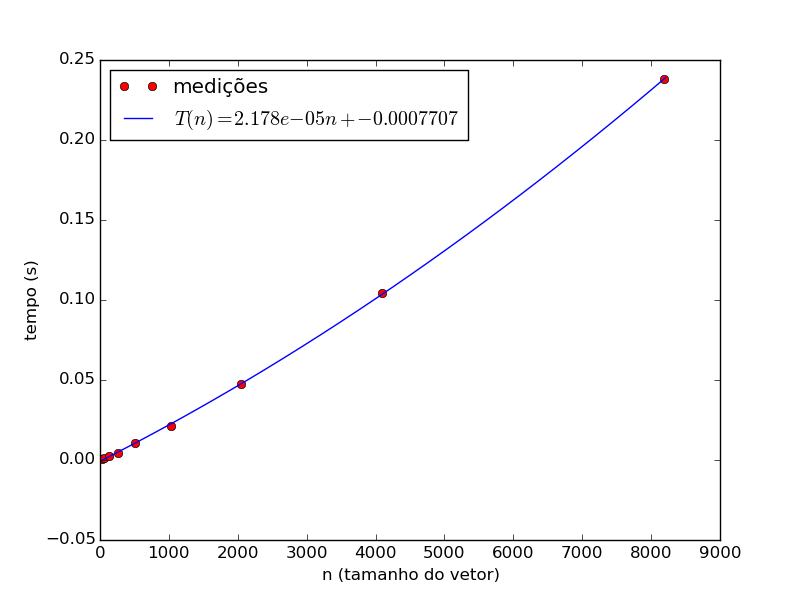
\includegraphics[scale=0.8]{../quicksort/imagens/quicksortAleatorio0.png}
\caption{A análise do grafico para $2^{32}$ segue abaixo para quicksort de vetor aleatório.}
Tendo a função $T(n) = 2.178\mathrm{e}-5*n-0.0007707$ e para o $n =2^{32}$, $T(2^{32}) = 93544.3869$ 
\label{fig:quicksortAleatorio0}
\end{figure}


\begin{figure}[ht]
\centering 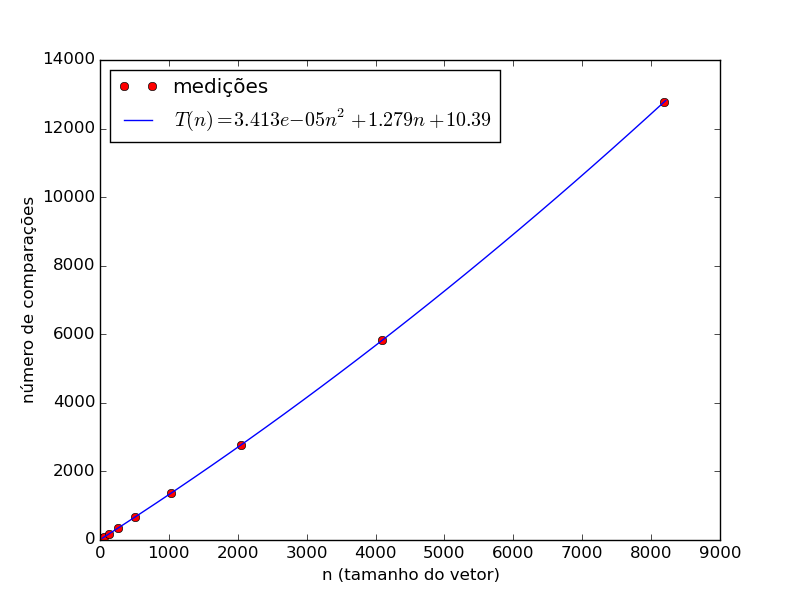
\includegraphics[scale=0.8]{../quicksort/imagens/quicksortAleatorio1.png}
\caption{A análise do grafico para $2^{32}$ segue abaixo para quicksort de vetor aleatório1.}
Tendo a função $T(n) = 3.413\mathrm{e}-5*n^2+1.279*n+10.39$ e para o $n =2^{32}$, $T(2^{32}) = 6.1355* 10^{303}$ 
\label{fig:quicksortAleatorio1}
\end{figure}


\begin{table}[ht]
\centering
\begin{tabular}{rrr} \toprule
        n &    comparações &       tempo(s) \\ \midrule
      32  &             45 &      0.000460 \\
      64  &             83 &      0.000982 \\
     128  &            169 &      0.002313 \\
     256  &            351 &      0.004588 \\
     512  &            679 &      0.010330 \\
    1024  &           1359 &      0.023083 \\
    2048  &           2743 &      0.047348 \\
    4096  &           4855 &      0.099813 \\
    8192  &          12431 &      0.220136 \\
\bottomrule\addlinespace
\end{tabular}
\caption{Tabela com vetor teste crescente: A linha te interesse analisada para este caso é a 12.}
\label{tab:quicksortCrescente}
\end{table}


\begin{figure}[ht]
\centering 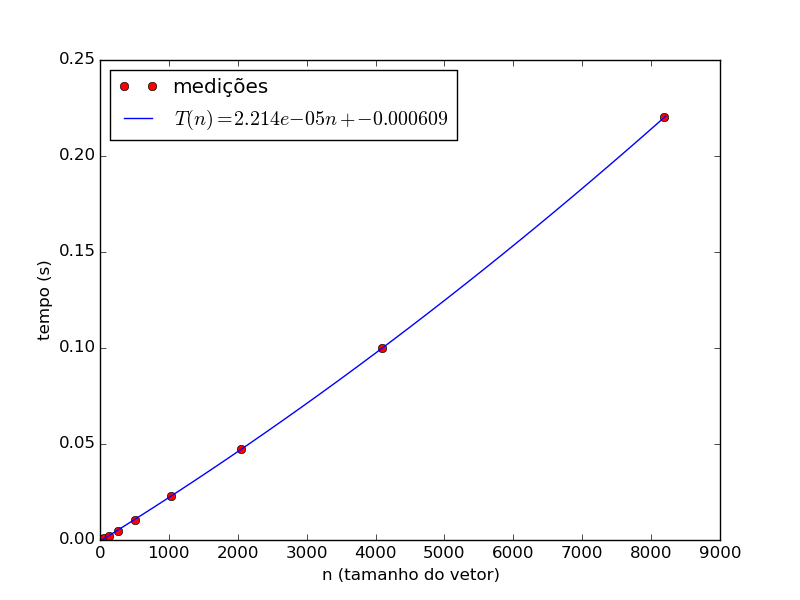
\includegraphics[scale=0.8]{../quicksort/imagens/quicksortCrescente0.png}
\caption{A análise do grafico para $2^{32}$ segue abaixo para quicksort de vetor crescente0}
Tendo a função $T(n) = 2.214\mathrm{e}-5*n-0.000609$ e para o $n =2^{32}$, $T(2^{32}) =  95090.57532444$ 
\label{fig:quicksortCrescente0}
\end{figure}

Tendo a função $T(n) = 2.214\mathrm{e}-5*n-0.000609$ e para o $n =2^{32}$, $T(2^{32}) = 95090.57532444$ 

\begin{figure}[ht]
\centering 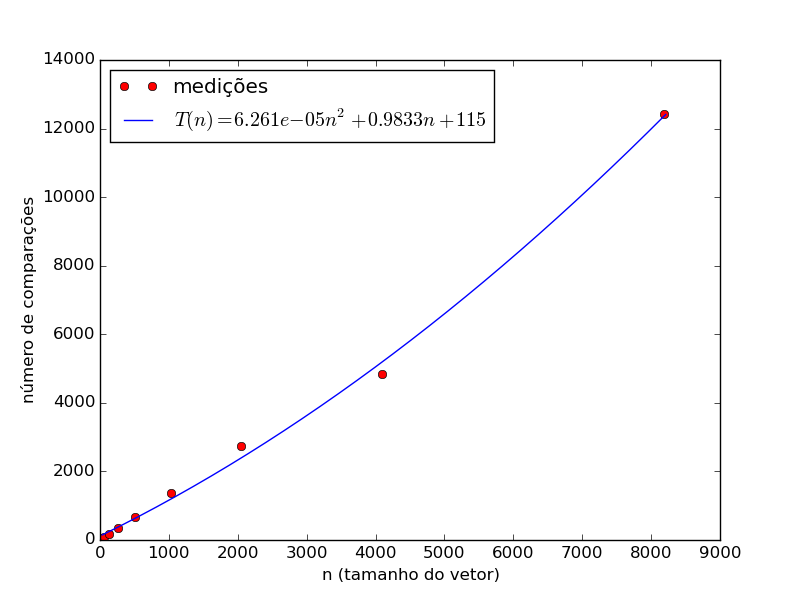
\includegraphics[scale=0.8]{../quicksort/imagens/quicksortCrescente1.png}
\caption{A análise do grafico para $2^{32}$ segue abaixo para quicksort de vetor crescente1}
Tendo a função $T(n) = 6.261\mathrm{e}-5*n^2+0.9833*n+155$ e para o $n =2^{32}$, $T(2^{32}) = 1.1255 * 10^{304}$ 

\label{fig:quicksortCrescente1}
\end{figure}


\begin{table}[ht]
\centering
\begin{tabular}{rrr} \toprule
        n &    comparações &       tempo(s) \\ \midrule
      32  &             41 &      0.000455 \\
      64  &             77 &      0.000949 \\
     128  &            169 &      0.002131 \\
     256  &            351 &      0.004956 \\
     512  &            685 &      0.009586 \\
    1024  &           1363 &      0.021693 \\
    2048  &           2753 &      0.045795 \\
    4096  &           4803 &      0.096253 \\
    8192  &          12439 &      0.230301 \\
\bottomrule\addlinespace
\end{tabular}
\caption{Tabela com vetor teste decrescente: A linha te interesse analisada para este caso é a 12.}
\label{tab:quicksortDecrescente}
\end{table}


\begin{figure}[ht]
\centering 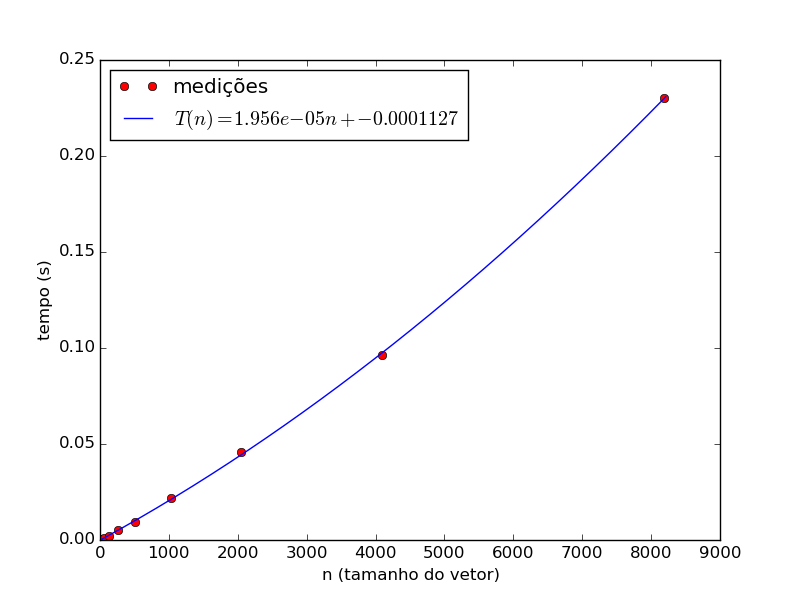
\includegraphics[scale=0.8]{../quicksort/imagens/quicksortDecrescente0.png}
\caption{A análise do grafico para $2^{32}$ segue abaixo para quicksort de vetor decrescente0}
Tendo a função $T(n) = 1.956\mathrm{e}-5*n-0.00001127$ e para o $n =2^{32}$, $T(2^{32}) = 84009.56029849$ 
\label{fig:quicksortDecrescente0}
\end{figure}

\begin{figure}[ht]
\centering 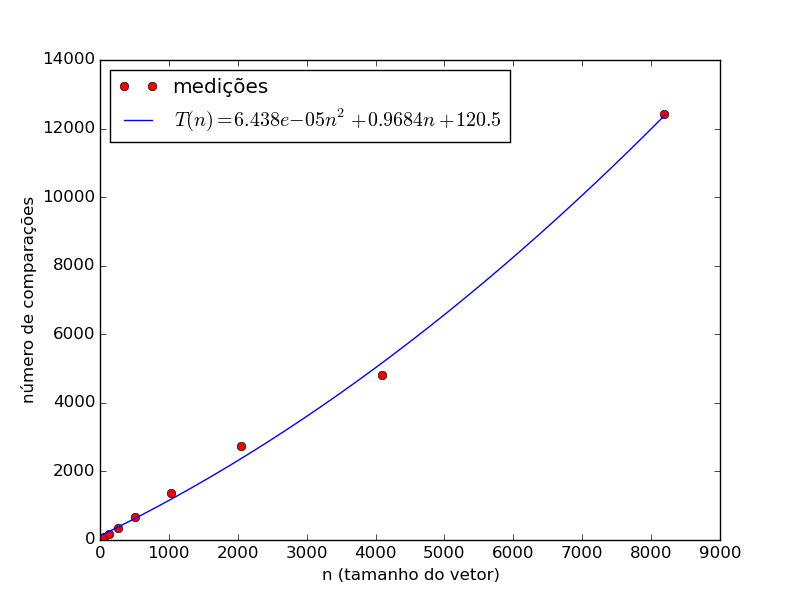
\includegraphics[scale=0.8]{../quicksort/imagens/quicksortDecrescente1.png}
\caption{A análise do grafico para $2^{32}$ segue abaixo para quicksort de vetor decrescente1}
Tendo a função $T(n) = 6.438\mathrm{e}-5*n^2+0.9684*n +120.5$ e para o $n =2^{32}$, $T(2^{32}) = 1.15735* 10^{304}$ 
\label{fig:quicksortDecrescente1}
\end{figure}


\begin{table}[ht]
\centering
\begin{tabular}{rrr} \toprule
        n &    comparações &       tempo(s) \\ \midrule
      32  &             41 &      0.000451 \\
      64  &             83 &      0.001014 \\
     128  &            169 &      0.002203 \\
     256  &            341 &      0.004529 \\
     512  &            691 &      0.010736 \\
    1024  &           1387 &      0.022258 \\
    2048  &           2725 &      0.048822 \\
    4096  &           4773 &      0.096224 \\
    8192  &          12435 &      0.236025 \\
\bottomrule\addlinespace
\end{tabular}
\caption{Tabela com vetor teste quase crescente 10\%: A linha te interesse analisada para este caso é a 12.}
\label{tab:quicksortQuaseCresc10}
\end{table}


\begin{figure}[ht]
\centering 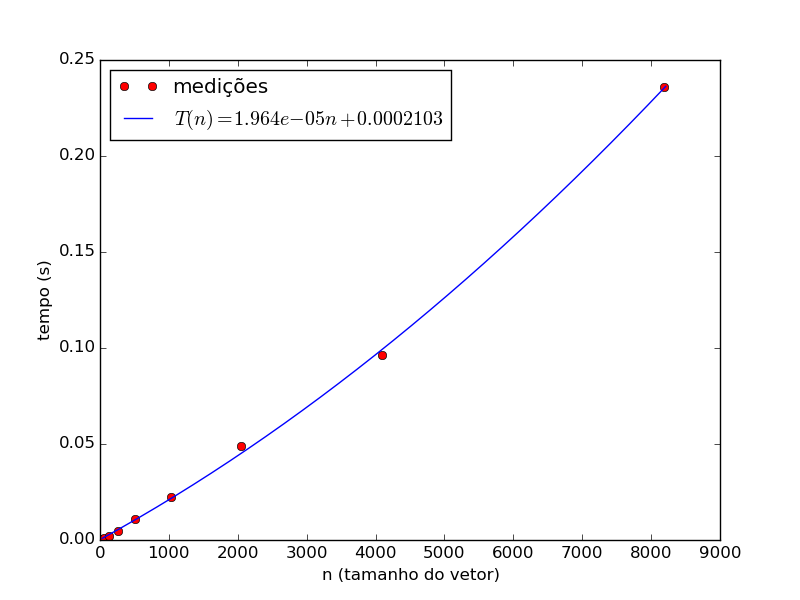
\includegraphics[scale=0.8]{../quicksort/imagens/quicksortQuaseCresc100.png}
\caption{A análise do grafico para $2^{32}$ segue abaixo para quicksort de vetor crescente100}
Tendo a função $T(n) = 1.964\mathrm{e}-5*n+0.0002103$ e para o $n =2^{32}$, $T(2^{32}) = 84353.15790374$ 
\label{fig:quicksortQuaseCresc100}
\end{figure}


\begin{figure}[ht]
\centering 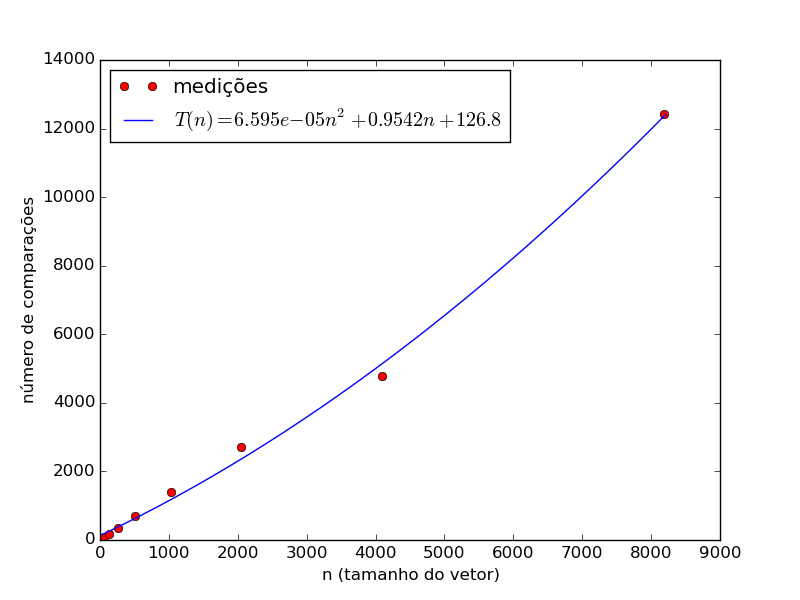
\includegraphics[scale=0.8]{../quicksort/imagens/quicksortQuaseCresc101.png}
\caption{A análise do grafico para $2^{32}$ segue abaixo para quicksort de vetor crescente101}

Tendo a função $T(n) = 6.595\mathrm{e}-5*n^2+0.9542*n+126.8$ e para o $n =2^{32}$, $T(2^{32}) = 1.1855*10^{304}$ 

\label{fig:quicksortQuaseCresc101}
\end{figure}


\begin{table}[ht]
\centering
\begin{tabular}{rrr} \toprule
        n &    comparações &       tempo(s) \\ \midrule
      32  &             41 &      0.000460 \\
      64  &             87 &      0.000899 \\
     128  &            165 &      0.002290 \\
     256  &            343 &      0.004409 \\
     512  &            691 &      0.010402 \\
    1024  &           1367 &      0.022453 \\
    2048  &           2735 &      0.048965 \\
    4096  &           4825 &      0.102515 \\
    8192  &          12433 &      0.236374 \\
\bottomrule\addlinespace
\end{tabular}
\caption{Tabela com vetor teste quase crescente 20\%: A linha te interesse analisada para este caso é a 12.}
\label{tab:quicksortQuaseCresc20}
\end{table}


\begin{figure}[ht]
\centering 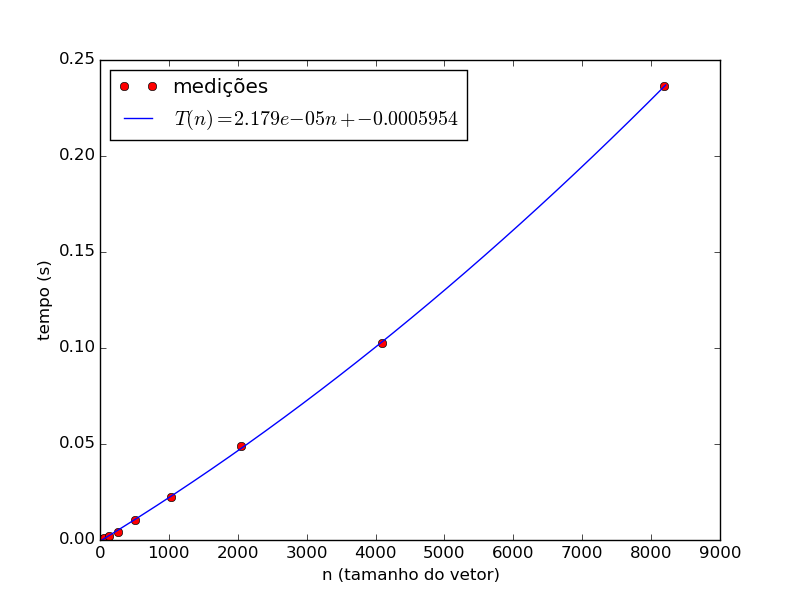
\includegraphics[scale=0.8]{../quicksort/imagens/quicksortQuaseCresc200.png}
\caption{A análise do grafico para $2^{32}$ segue abaixo para quicksort de vetor crescente200}
Tendo a função $T(n) = 2.179\mathrm{e}-5*n-0.0005954$ e para o $n =2^{32}$, $T(2^{32}) = 93587.33678444$ 

\label{fig:quicksortQuaseCresc200}
\end{figure}

\begin{figure}[ht]
\centering 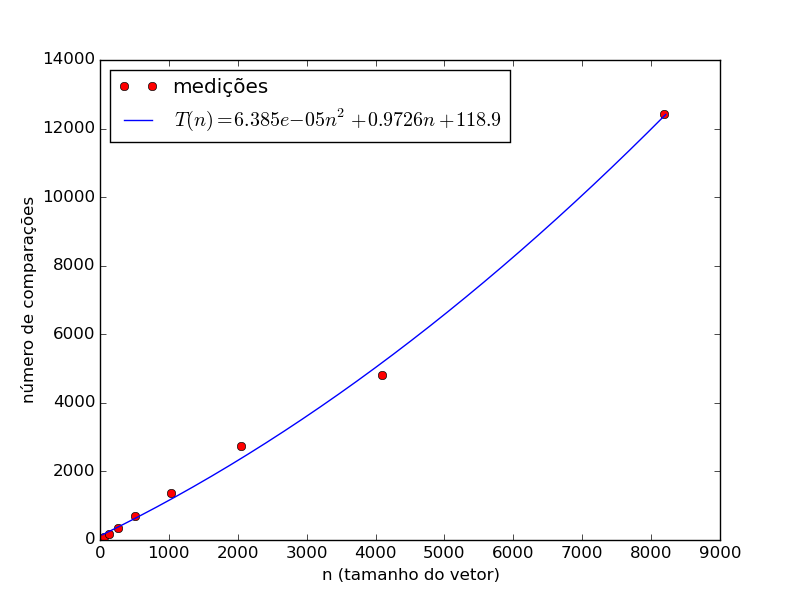
\includegraphics[scale=0.8]{../quicksort/imagens/quicksortQuaseCresc201.png}
\caption{A análise do grafico para $2^{32}$ segue abaixo para quicksort de vetor crescente201}
Tendo a função $T(n) = 6.385\mathrm{e}-5*n^2+0.9726*n+111.9$ e para o $n =2^{32}$, $T(2^{32}) = 1.14782*10^{304}$ 
\label{fig:quicksortQuaseCresc201}
\end{figure}

\clearpage
\begin{table}[ht]
\centering
\begin{tabular}{rrr} \toprule
        n &    comparações &       tempo(s) \\ \midrule
      32  &             41 &      0.000418 \\
      64  &             81 &      0.000956 \\
     128  &            169 &      0.002140 \\
     256  &            349 &      0.004458 \\
     512  &            687 &      0.009880 \\
    1024  &           1371 &      0.020995 \\
    2048  &           2737 &      0.051357 \\
    4096  &           4875 &      0.101185 \\
    8192  &          12439 &      0.238561 \\
\bottomrule\addlinespace
\end{tabular}
\caption{Tabela com vetor teste quase crescente 30\%: A linha te interesse analisada para este caso é a 12.}
\label{tab:quicksortQuaseCresc30}
\end{table}


\begin{figure}[ht]
\centering 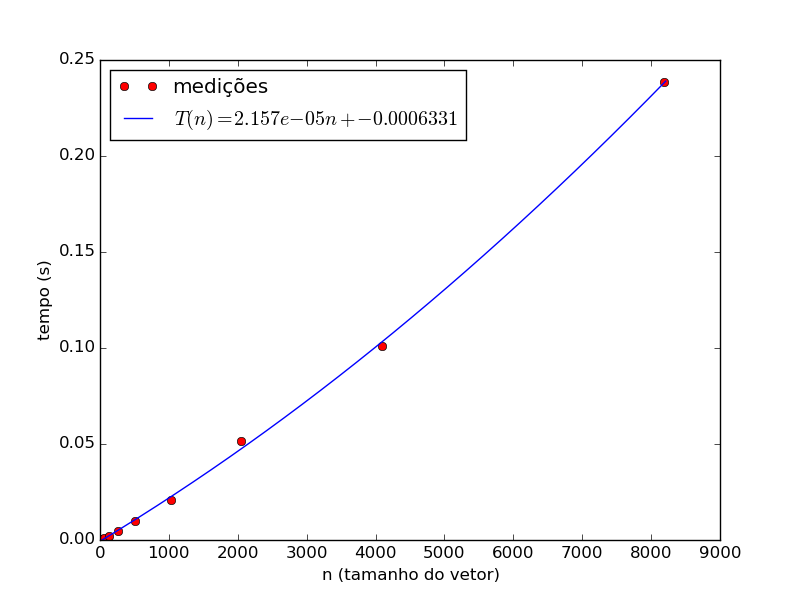
\includegraphics[scale=0.8]{../quicksort/imagens/quicksortQuaseCresc300.png}
\caption{A análise do grafico para $2^{32}$ segue abaixo para quicksort de vetor crescente300}
Tendo a função $T(n) = 2.157\mathrm{e}-5*n-0.0006331$ e para o $n =2^{32}$, $T(2^{32}) = 92642.44394162$ 
\label{fig:quicksortQuaseCresc300}
\end{figure}

\begin{figure}[ht]
\centering 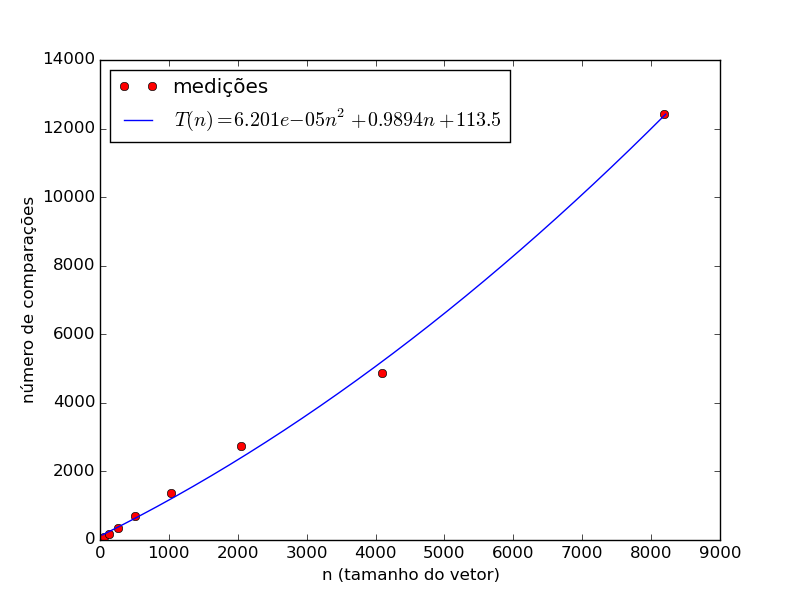
\includegraphics[scale=0.8]{../quicksort/imagens/quicksortQuaseCresc301.png}
\caption{A análise do grafico para $2^{32}$ segue abaixo para quicksort de vetor crescente301}

Tendo a função $T(n) = 6.201\mathrm{e}-5*n^2 + 0.9894*n+113.5$ e para o $n =2^{32}$, $T(2^{32}) = 1.1438 × 10^{15}$ 

\label{fig:quicksortQuaseCresc301}
\end{figure}


\begin{table}[ht]
\centering
\begin{tabular}{rrr} \toprule
        n &    comparações &       tempo(s) \\ \midrule
      32  &             45 &      0.000475 \\
      64  &             91 &      0.001001 \\
     128  &            175 &      0.002174 \\
     256  &            341 &      0.004848 \\
     512  &            679 &      0.010063 \\
    1024  &           1391 &      0.021854 \\
    2048  &           2737 &      0.046297 \\
    4096  &           4797 &      0.097154 \\
    8192  &          12429 &      0.247491 \\
\bottomrule\addlinespace
\end{tabular}
\caption{Tabela com vetor teste quase crescente 40\%: A linha te interesse analisada para este caso é a 12.}
\label{tab:quicksortQuaseCresc40}
\end{table}


\begin{figure}[ht]
\centering 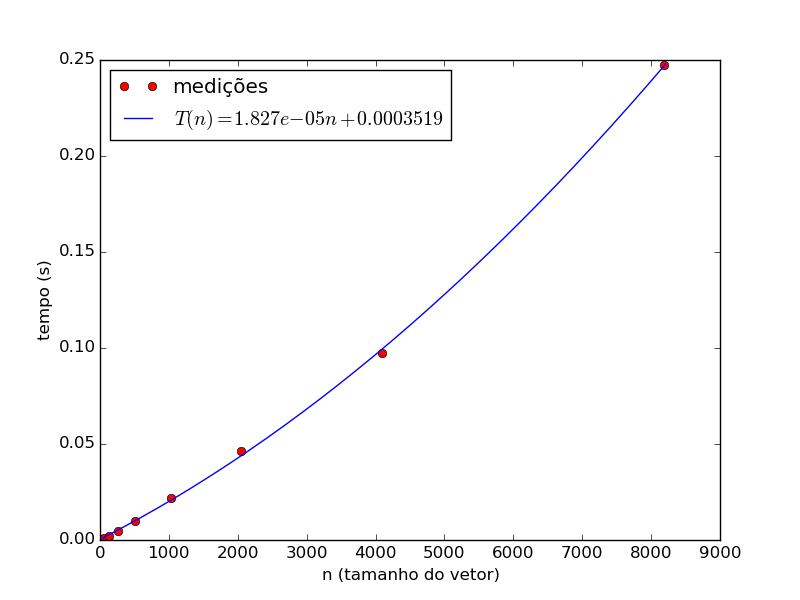
\includegraphics[scale=0.8]{../quicksort/imagens/quicksortQuaseCresc400.png}
\caption{A análise do grafico para $2^{32}$ segue abaixo para quicksort de vetor crescente400}

Tendo a função $T(n) = 1.827\mathrm{e}-5*n+0.0003519$ e para o $n =2^{32}$, $T(2^{32}) = 78469.05284982$ 

\label{fig:quicksortQuaseCresc400}
\end{figure}

\begin{figure}[ht]
\centering 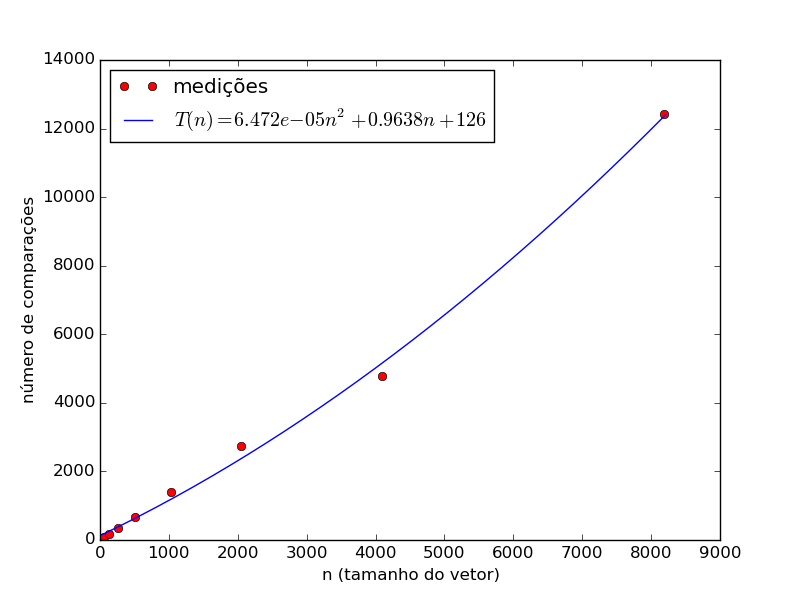
\includegraphics[scale=0.8]{../quicksort/imagens/quicksortQuaseCresc401.png}
\caption{A análise do grafico para $2^{32}$ segue abaixo para quicksort de vetor crescente401}
Tendo a função $T(n) = 6.472\mathrm{e}-5*n^2+0.9638*n+126$ e para o $n =2^{32}$, $T(2^{32}) = 1.1634 × 10^{304}$ 

\label{fig:quicksortQuaseCresc401}
\end{figure}


\begin{table}[ht]
\centering
\begin{tabular}{rrr} \toprule
        n &    comparações &       tempo(s) \\ \midrule
      32  &             47 &      0.000495 \\
      64  &             89 &      0.001033 \\
     128  &            175 &      0.002108 \\
     256  &            357 &      0.004774 \\
     512  &            671 &      0.009816 \\
    1024  &           1357 &      0.023627 \\
    2048  &           2743 &      0.046188 \\
    4096  &           4851 &      0.098774 \\
    8192  &          12439 &      0.234423 \\
\bottomrule\addlinespace
\end{tabular}
\caption{Tabela com vetor teste quase crescente 50\%: A linha te interesse analisada para este caso é a 12.}
\label{tab:quicksortQuaseCresc50}
\end{table}


\begin{figure}[ht]
\centering 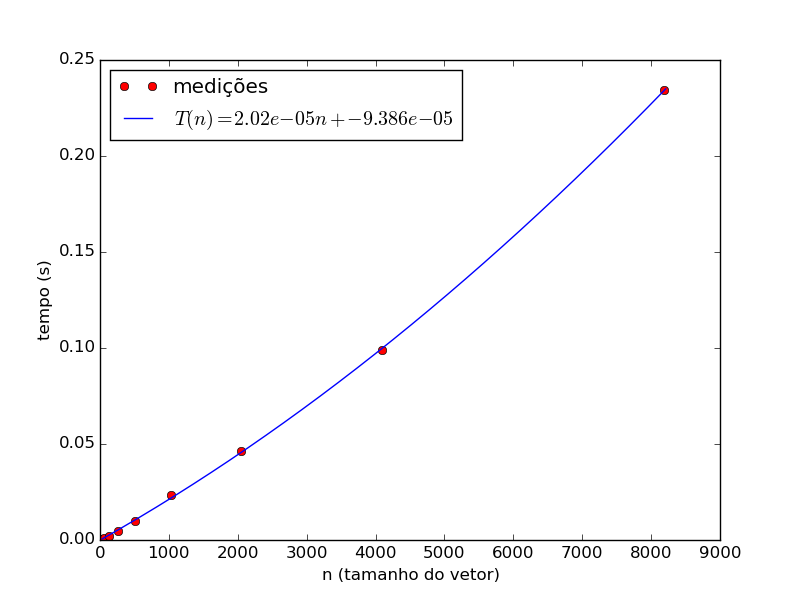
\includegraphics[scale=0.8]{../quicksort/imagens/quicksortQuaseCresc500.png}
\caption{A análise do grafico para $2^{32}$ segue abaixo para quicksort de vetor crescente500}

Tendo a função $T(n) = 2.02\mathrm{e}-5*n-9.386\mathrm{e}-05$ e para o $n =2^{32}$, $T(2^{32}) = 86758.33928534$ 

\label{fig:quicksortQuaseCresc500}
\end{figure}

\begin{figure}[ht]
\centering 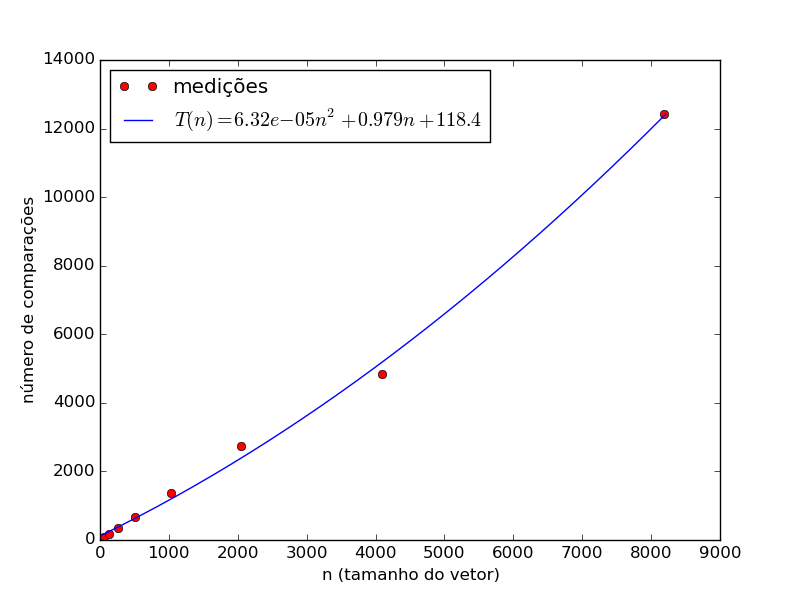
\includegraphics[scale=0.8]{../quicksort/imagens/quicksortQuaseCresc501.png}
\caption{A análise do grafico para $2^{32}$ segue abaixo para quicksort de vetor crescente501}

Tendo a função $T(n) = 6.32\mathrm{e}-5*n^2+0.979*n+118.4$ e para o $n =2^{32}$, $T(2^{32}) = 1.13614*10^{304}$ 

\label{fig:quicksortQuaseCresc501}
\end{figure}


\begin{table}[ht]
\centering
\begin{tabular}{rrr} \toprule
        n &    comparações &       tempo(s) \\ \midrule
      32  &             43 &      0.000497 \\
      64  &             87 &      0.000969 \\
     128  &            169 &      0.002212 \\
     256  &            343 &      0.005239 \\
     512  &            687 &      0.009943 \\
    1024  &           1387 &      0.023199 \\
    2048  &           2761 &      0.048857 \\
    4096  &           4829 &      0.100816 \\
    8192  &          12431 &      0.230520 \\
\bottomrule\addlinespace
\end{tabular}
\caption{Tabela com vetor teste quase decrescente 10\%: A linha te interesse analisada para este caso é a 12.}
\label{tab:quicksortQuaseDecresc10}
\end{table}


\begin{figure}[ht]
\centering 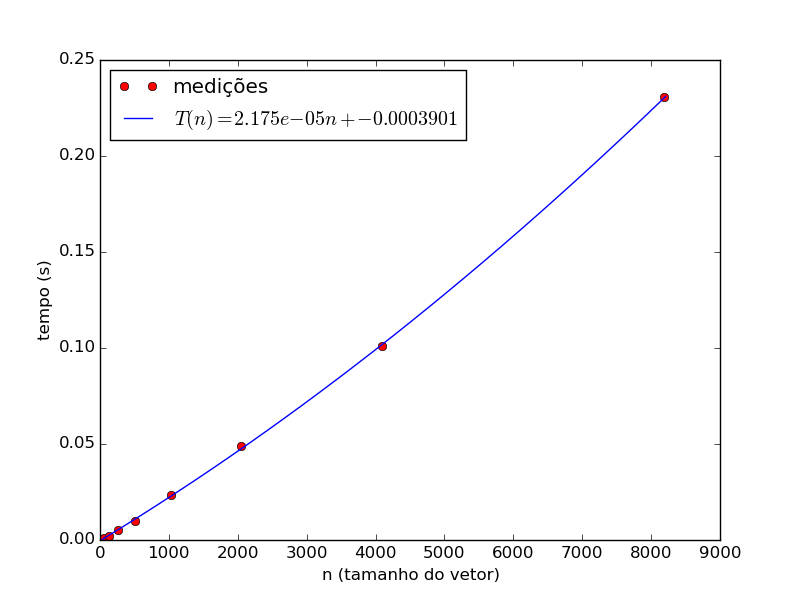
\includegraphics[scale=0.8]{../quicksort/imagens/quicksortQuaseDecresc100.png}
\caption{A análise do grafico para $2^{32}$ segue abaixo para quicksort de vetor decrescente100}

Tendo a função $T(n) = 2.175\mathrm{e}-5*n - 0.0003901$ e para o $n =2^{32}$, $T(2^{32}) = 93415.5382$ 

\label{fig:quicksortQuaseDecresc100}
\end{figure}

\begin{figure}[ht]
\centering 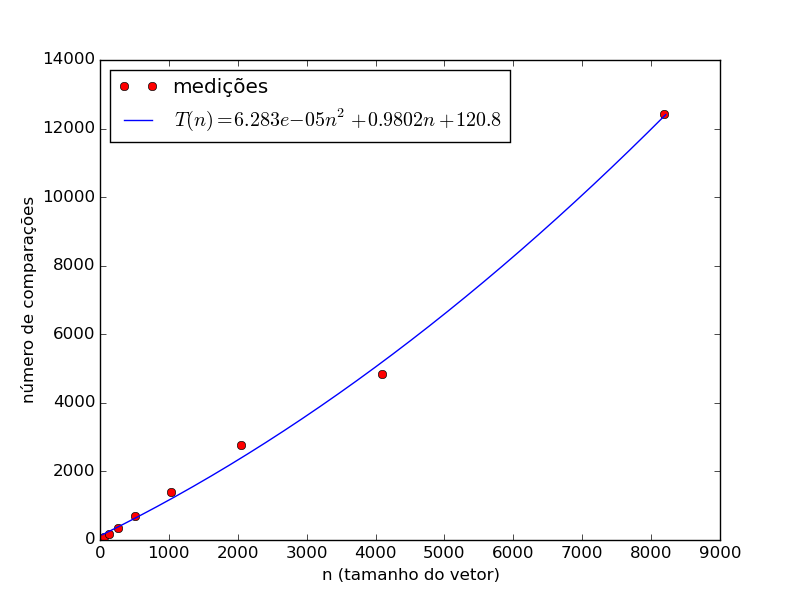
\includegraphics[scale=0.8]{../quicksort/imagens/quicksortQuaseDecresc101.png}
\caption{A análise do grafico para $2^{32}$ segue abaixo para quicksort de vetor decrescente101}


Tendo a função $T(n) = 6.283\mathrm{e}-5*n^2+0.9802*n+120.8$ e para o $n =2^{32}$, $T(2^{32}) = 4.75507*10^{313}$ 

\label{fig:quicksortQuaseDecresc101}
\end{figure}


\begin{table}[ht]
\centering
\begin{tabular}{rrr} \toprule
        n &    comparações &       tempo(s) \\ \midrule
      32  &             45 &      0.000498 \\
      64  &             87 &      0.001026 \\
     128  &            165 &      0.002288 \\
     256  &            341 &      0.004596 \\
     512  &            687 &      0.010886 \\
    1024  &           1339 &      0.025004 \\
    2048  &           2713 &      0.050401 \\
    4096  &           4825 &      0.095543 \\
    8192  &          12433 &      0.237404 \\
\bottomrule\addlinespace
\end{tabular}
\caption{Tabela com vetor teste quase decrescente 20\%: A linha te interesse analisada para este caso é a 12.}
\label{tab:quicksortQuaseDecresc20}
\end{table}


\begin{figure}[ht]
\centering 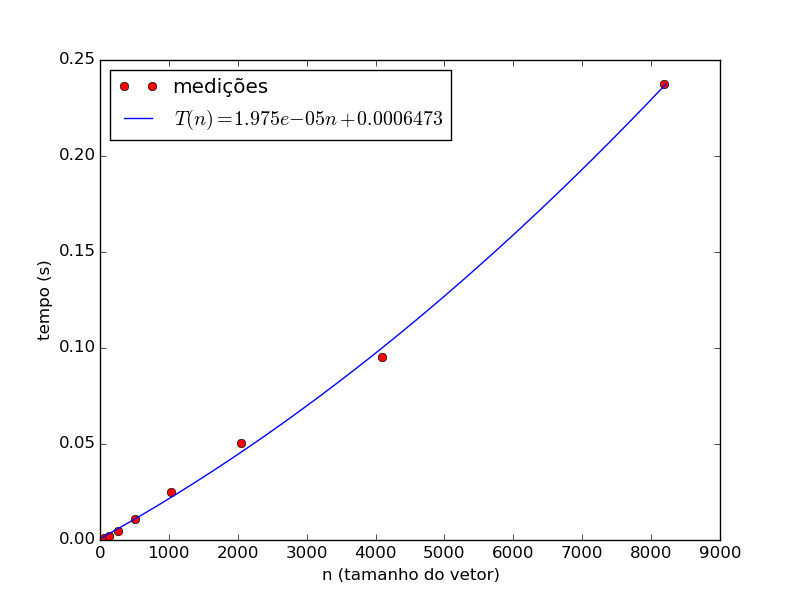
\includegraphics[scale=0.8]{../quicksort/imagens/quicksortQuaseDecresc200.png}
\caption{A análise do grafico para $2^{32}$ segue abaixo para quicksort de vetor decrescente101}

Tendo a função $T(n) = 1.975\mathrm{e}-5*n+0.0006473$ e para o $n =2^{32}$, $T(2^{32}) = 84825.6047433$ 

\label{fig:quicksortQuaseDecresc200}
\end{figure}

\begin{figure}[ht]
\centering 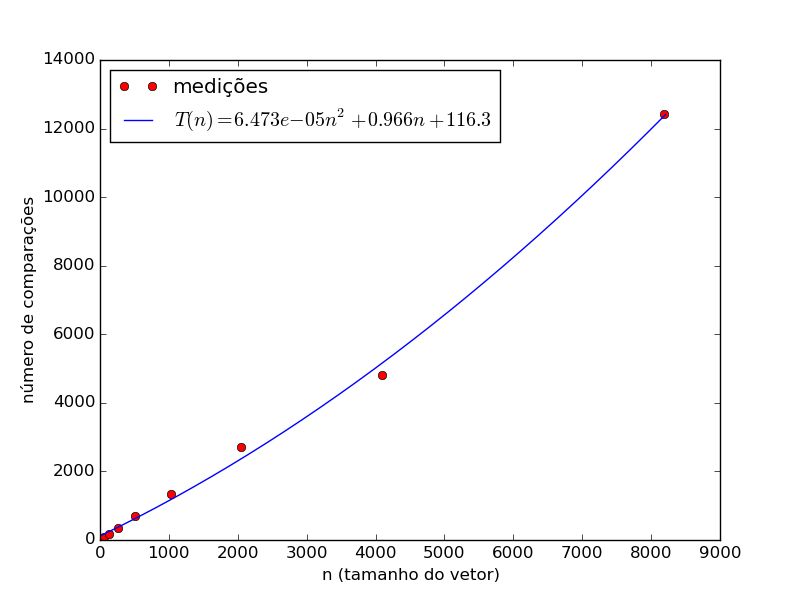
\includegraphics[scale=0.8]{../quicksort/imagens/quicksortQuaseDecresc201.png}
\caption{A análise do grafico para $2^{32}$ segue abaixo para quicksort de vetor decrescente201}

Tendo a função $T(n) = 6.473\mathrm{e}-5*n^2+0.966*n + 116.3$ e para o $n =2^{32}$, $T(2^{32}) = 84825.6047433$ 

\label{fig:quicksortQuaseDecresc201}
\end{figure}

\clearpage
\begin{table}[ht]
\centering
\begin{tabular}{rrr} \toprule
        n &    comparações &       tempo(s) \\ \midrule
      32  &             45 &      0.000490 \\
      64  &             81 &      0.000922 \\
     128  &            179 &      0.002251 \\
     256  &            347 &      0.004792 \\
     512  &            695 &      0.009644 \\
    1024  &           1361 &      0.022657 \\
    2048  &           2735 &      0.047662 \\
    4096  &           4841 &      0.095222 \\
    8192  &          12441 &      0.236857 \\
\bottomrule\addlinespace
\end{tabular}
\caption{Tabela com vetor teste quase decrescente 30\%: A linha te interesse analisada para este caso é a 12.}
\label{tab:quicksortQuaseDecresc30}
\end{table}


\begin{figure}[ht]
\centering 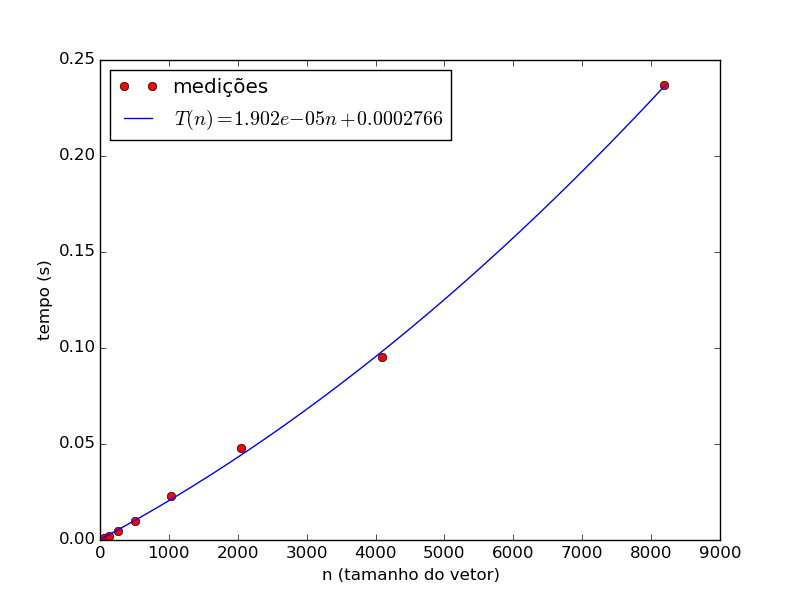
\includegraphics[scale=0.8]{../quicksort/imagens/quicksortQuaseDecresc300.png}
\caption{A análise do grafico para $2^{32}$ segue abaixo para quicksort de vetor decrescente300}

Tendo a função $T(n) = 1.902\mathrm{e}-5*n+0.0002766$ e para o $n =2^{32}$, $T(2^{32}) = 81690.27824652$ 

\label{fig:quicksortQuaseDecresc300}
\end{figure}

\begin{figure}[ht]
\centering 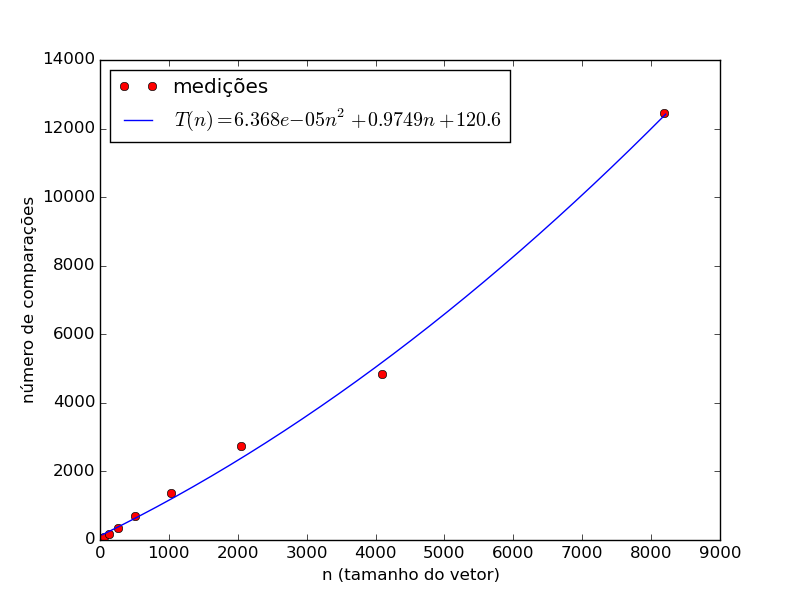
\includegraphics[scale=0.8]{../quicksort/imagens/quicksortQuaseDecresc301.png}
\caption{A análise do grafico para $2^{32}$ segue abaixo para quicksort de vetor decrescente301}

Tendo a função $T(n) = 6.368\mathrm{e}-5*n+120.6$ e para o $n =2^{32}$, $T(2^{32}) = 273624.11740928$ 

\label{fig:quicksortQuaseDecresc301}
\end{figure}


\begin{table}[ht]
\centering
\begin{tabular}{rrr} \toprule
        n &    comparações &       tempo(s) \\ \midrule
      32  &             41 &      0.000448 \\
      64  &             89 &      0.000929 \\
     128  &            171 &      0.002126 \\
     256  &            331 &      0.004763 \\
     512  &            689 &      0.010562 \\
    1024  &           1367 &      0.023329 \\
    2048  &           2697 &      0.047045 \\
    4096  &           4859 &      0.094538 \\
    8192  &          12435 &      0.232884 \\
\bottomrule\addlinespace
\end{tabular}
\caption{Tabela com vetor teste quase decrescente 40\%: A linha te interesse analisada para este caso é a 12.}
\label{tab:quicksortQuaseDecresc40}
\end{table}


\begin{figure}[ht]
\centering 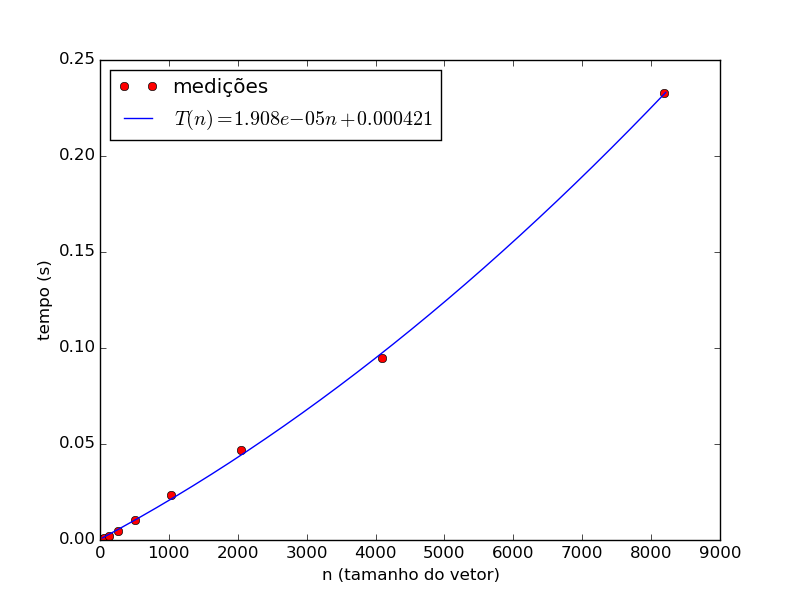
\includegraphics[scale=0.8]{../quicksort/imagens/quicksortQuaseDecresc400.png}
\caption{A análise do grafico para $2^{32}$ segue abaixo para quicksort de vetor decrescente400}

Tendo a função $T(n) = 1.908\mathrm{e}-5*n+0.000421$ e para o $n =2^{32}$, $T(2^{32}) = 81947.97642868$ 

\label{fig:quicksortQuaseDecresc400}
\end{figure}

\begin{figure}[ht]
\centering 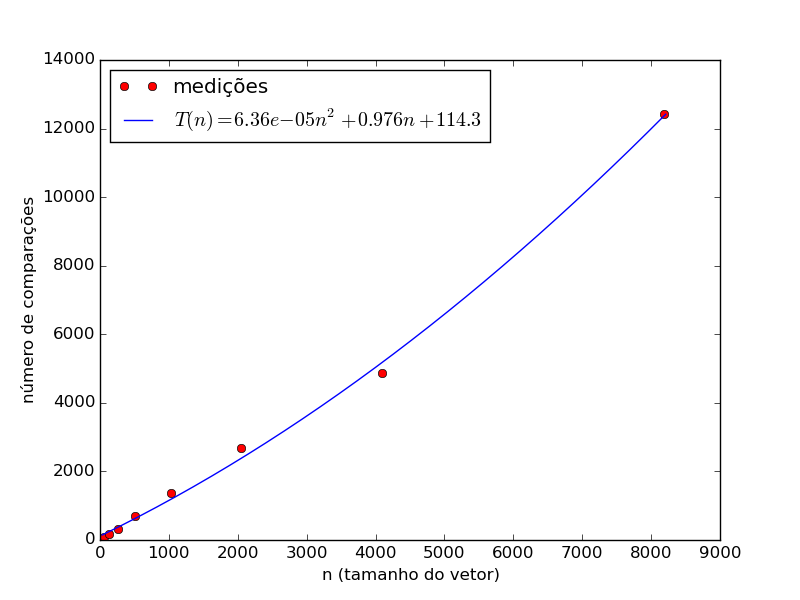
\includegraphics[scale=0.8]{../quicksort/imagens/quicksortQuaseDecresc401.png}
\caption{A análise do grafico para $2^{32}$ segue abaixo para quicksort de vetor decrescente401}

Tendo a função $T(n) = 6.36\mathrm{e}-5*n+0.976*n+114.3$ e para o $n =2^{32}$, $T(2^{32}) = 4.1921*10^9$

\label{fig:quicksortQuaseDecresc401}
\end{figure}


\begin{table}[ht]
\centering
\begin{tabular}{rrr} \toprule
        n &    comparações &       tempo(s) \\ \midrule
      32  &             47 &      0.000458 \\
      64  &             87 &      0.001033 \\
     128  &            177 &      0.002219 \\
     256  &            337 &      0.004370 \\
     512  &            675 &      0.010310 \\
    1024  &           1363 &      0.022362 \\
    2048  &           2737 &      0.048213 \\
    4096  &           4839 &      0.101969 \\
    8192  &          12435 &      0.230613 \\
\bottomrule\addlinespace
\end{tabular}
\caption{Tabela com vetor teste quase decrescente 50\%: A linha te interesse analisada para este caso é a 12.}
\label{tab:quicksortQuaseDecresc50}
\end{table}


\begin{figure}[ht]
\centering 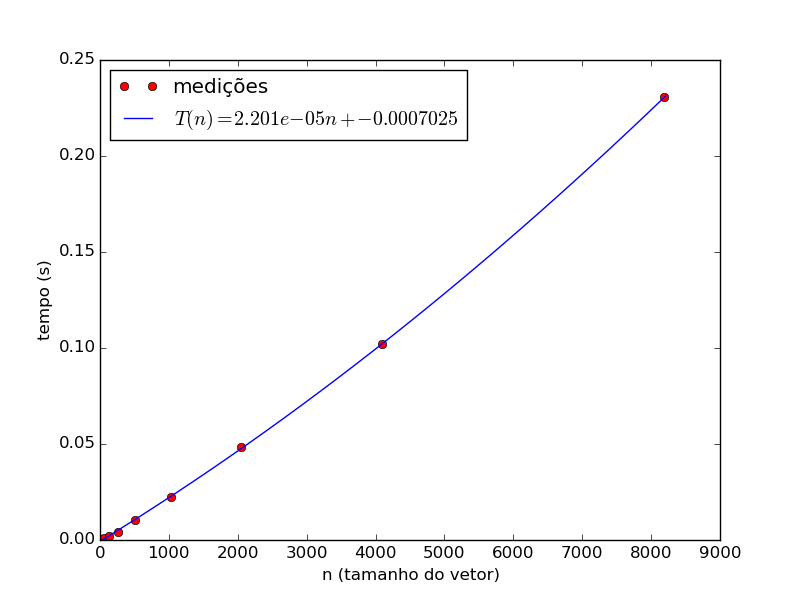
\includegraphics[scale=0.8]{../quicksort/imagens/quicksortQuaseDecresc500.png}
\caption{A análise do grafico para $2^{32}$ segue abaixo para quicksort de vetor decrescente500}

Tendo a função $T(n) = 2.201\mathrm{e}-5*n-0.0007025$ e para o $n =2^{32}$, $T(2^{32}) = 94532.22948246$

\label{fig:quicksortQuaseDecresc500}
\end{figure}

\begin{figure}[ht]
\centering 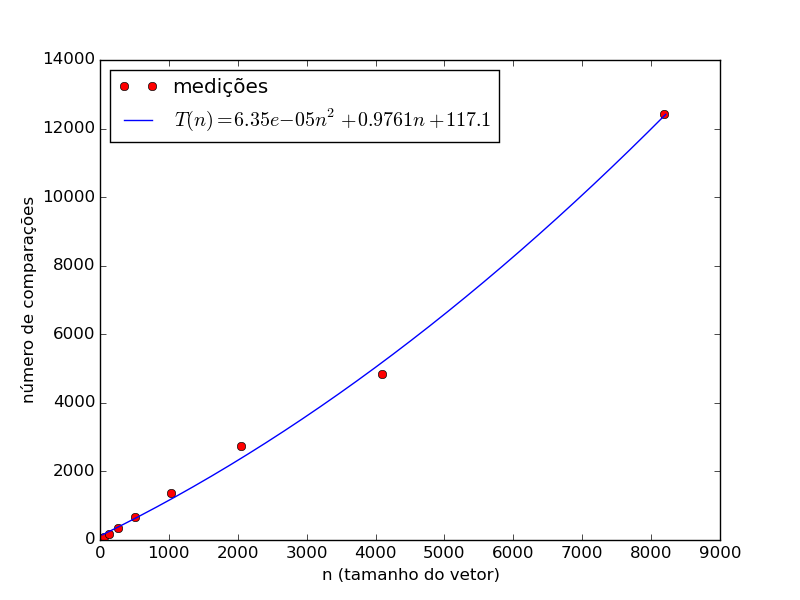
\includegraphics[scale=0.8]{../quicksort/imagens/quicksortQuaseDecresc501.png}
\caption{A análise do grafico para $2^{32}$ segue abaixo para quicksort de vetor decrescente501}

Tendo a função $T(n) = 6.35\mathrm{e}-5*n^2+0.9761*n+117.1$ e para o $n =2^{32}$, $T(2^{32}) = 1.141535*10^{304}$

\label{fig:quicksortQuaseDecresc501}
\end{figure}


\clearpage
\clearpage
\addcontentsline{toc}{part}{Apêndice}
\appendix

\chapter{Arquivo ../quicksort/quicksort.py \label{ap:quicksort}}
\lstinputlisting[caption={../quicksort/quicksort.py \label{arq:quicksort}}]{../quicksort/quicksort.py}

\chapter{Arquivo ../quicksort/ensaio.py \label{ap:quicksortensaio}}
\lstinputlisting[caption={../quicksort/ensaio.py \label{arq:quicksortensaio}}]{../quicksort/ensaio.py}

\end{document}
